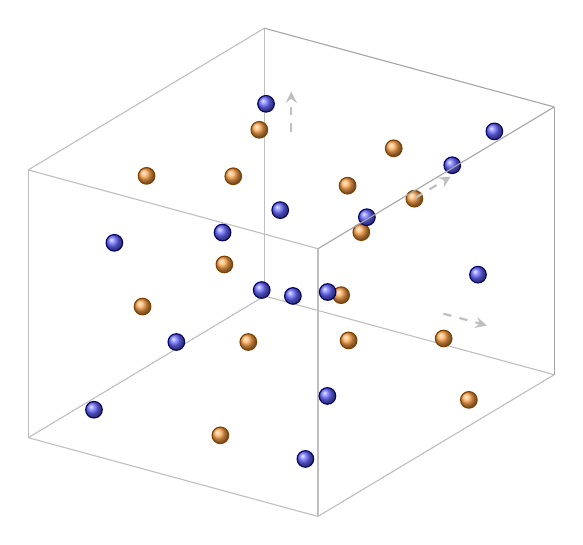
\begin{tikzpicture}[
    x={(0.92cm,-0.25cm)},
    y={(0.75cm,0.45cm)},
    z={(0cm,0.85cm)},
    ti/.style={circle, ball color=blue!60, draw=blue!40!black, minimum size=6pt, inner sep=0pt},
    al/.style={circle, ball color=orange!70, draw=orange!50!black, minimum size=6pt, inner sep=0pt},
]

% Box size
\def\L{4}

% Draw back edges (behind atoms)
\draw[gray!50, thin] (0,0,0) -- (\L,0,0);
\draw[gray!50, thin] (0,0,0) -- (0,\L,0);
\draw[gray!50, thin] (0,0,0) -- (0,0,\L);
\draw[gray!50, thin] (\L,0,0) -- (\L,\L,0);
\draw[gray!50, thin] (\L,0,0) -- (\L,0,\L);
\draw[gray!50, thin] (0,\L,0) -- (\L,\L,0);
\draw[gray!50, thin] (0,\L,0) -- (0,\L,\L);
\draw[gray!50, thin] (0,0,\L) -- (\L,0,\L);
\draw[gray!50, thin] (0,0,\L) -- (0,\L,\L);

% Atoms — scattered in the cell, mix of Ti and Al
% Layer 1 (low z)
\node[ti] at (0.5,0.5,0.3) {};
\node[al] at (2.0,0.8,0.2) {};
\node[ti] at (3.5,0.4,0.5) {};
\node[al] at (1.0,2.5,0.4) {};
\node[ti] at (2.5,2.0,0.3) {};
\node[al] at (3.8,2.8,0.2) {};
\node[ti] at (0.8,3.5,0.5) {};
\node[al] at (2.8,3.6,0.4) {};

% Layer 2 (mid z)
\node[al] at (0.6,1.2,1.5) {};
\node[ti] at (1.8,0.3,1.8) {};
\node[al] at (3.2,1.5,1.6) {};
\node[ti] at (0.4,2.8,1.7) {};
\node[al] at (2.2,2.6,1.4) {};
\node[ti] at (3.6,3.2,1.8) {};
\node[al] at (1.5,3.8,1.5) {};
\node[ti] at (2.0,1.5,2.0) {};

% Layer 3 (high z)
\node[ti] at (0.7,0.6,2.8) {};
\node[al] at (2.3,0.5,3.0) {};
\node[ti] at (3.4,0.9,2.7) {};
\node[al] at (1.2,2.0,3.2) {};
\node[ti] at (2.8,2.3,2.9) {};
\node[al] at (0.5,3.3,3.0) {};
\node[ti] at (3.0,3.5,3.1) {};
\node[al] at (1.8,3.2,2.6) {};

% Layer 4 (top z)
\node[al] at (0.9,0.9,3.7) {};
\node[ti] at (2.5,1.2,3.5) {};
\node[al] at (3.7,2.0,3.6) {};
\node[ti] at (1.0,2.8,3.8) {};
\node[al] at (2.6,3.0,3.5) {};
\node[ti] at (3.5,3.6,3.7) {};

% Front edges (on top of atoms)
\draw[gray!70, thin] (\L,\L,0) -- (\L,\L,\L);
\draw[gray!70, thin] (\L,0,\L) -- (\L,\L,\L);
\draw[gray!70, thin] (0,\L,\L) -- (\L,\L,\L);

% Periodic boundary hint: dashed arrows
\draw[->, >=stealth, dashed, gray!50, thick] (\L+0.1,2,2) -- (\L+0.7,2,2);
\draw[->, >=stealth, dashed, gray!50, thick] (2,\L+0.1,2) -- (2,\L+0.7,2);
\draw[->, >=stealth, dashed, gray!50, thick] (2,2,\L+0.1) -- (2,2,\L+0.7);

\end{tikzpicture}
